\subsection{R and Python scripts} \label{r_scripts}

\subsubsection{Correlation between temperature and conductivity}
\Rfile{scripts/lfk_temp.R}

\newpage
\subsubsection{Molar conductivity of different electrolytes}
\Rfile{scripts/lfk_molar.R}

\newpage
\subsubsection{Conductometric titration}
\Rfile{scripts/lfk_titr.R}

\newpage
\subsubsection{Plotting helper scripts}
\Rfile{scripts/helpers.R}

\begin{figure}[H]
    \centering
    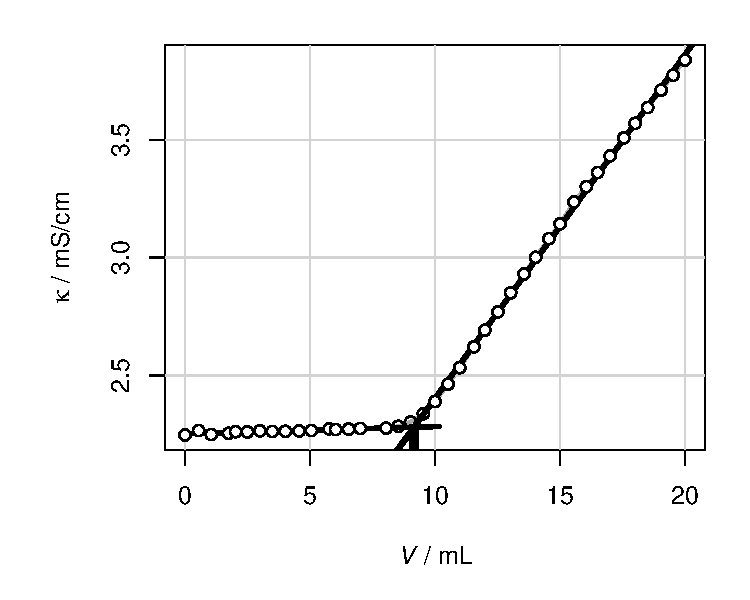
\includegraphics[width=.9\textwidth]{figures/plots/lfk_titration_full.pdf}
    \caption{Full view of the titration of $\mathrm{K_{2}CO_{3}}$ with \qty[round-precision=5]{0.09997}{\M} $\mathrm{CaCl_2}$.}
    \label{fig:lfk_titr_full}
\end{figure}

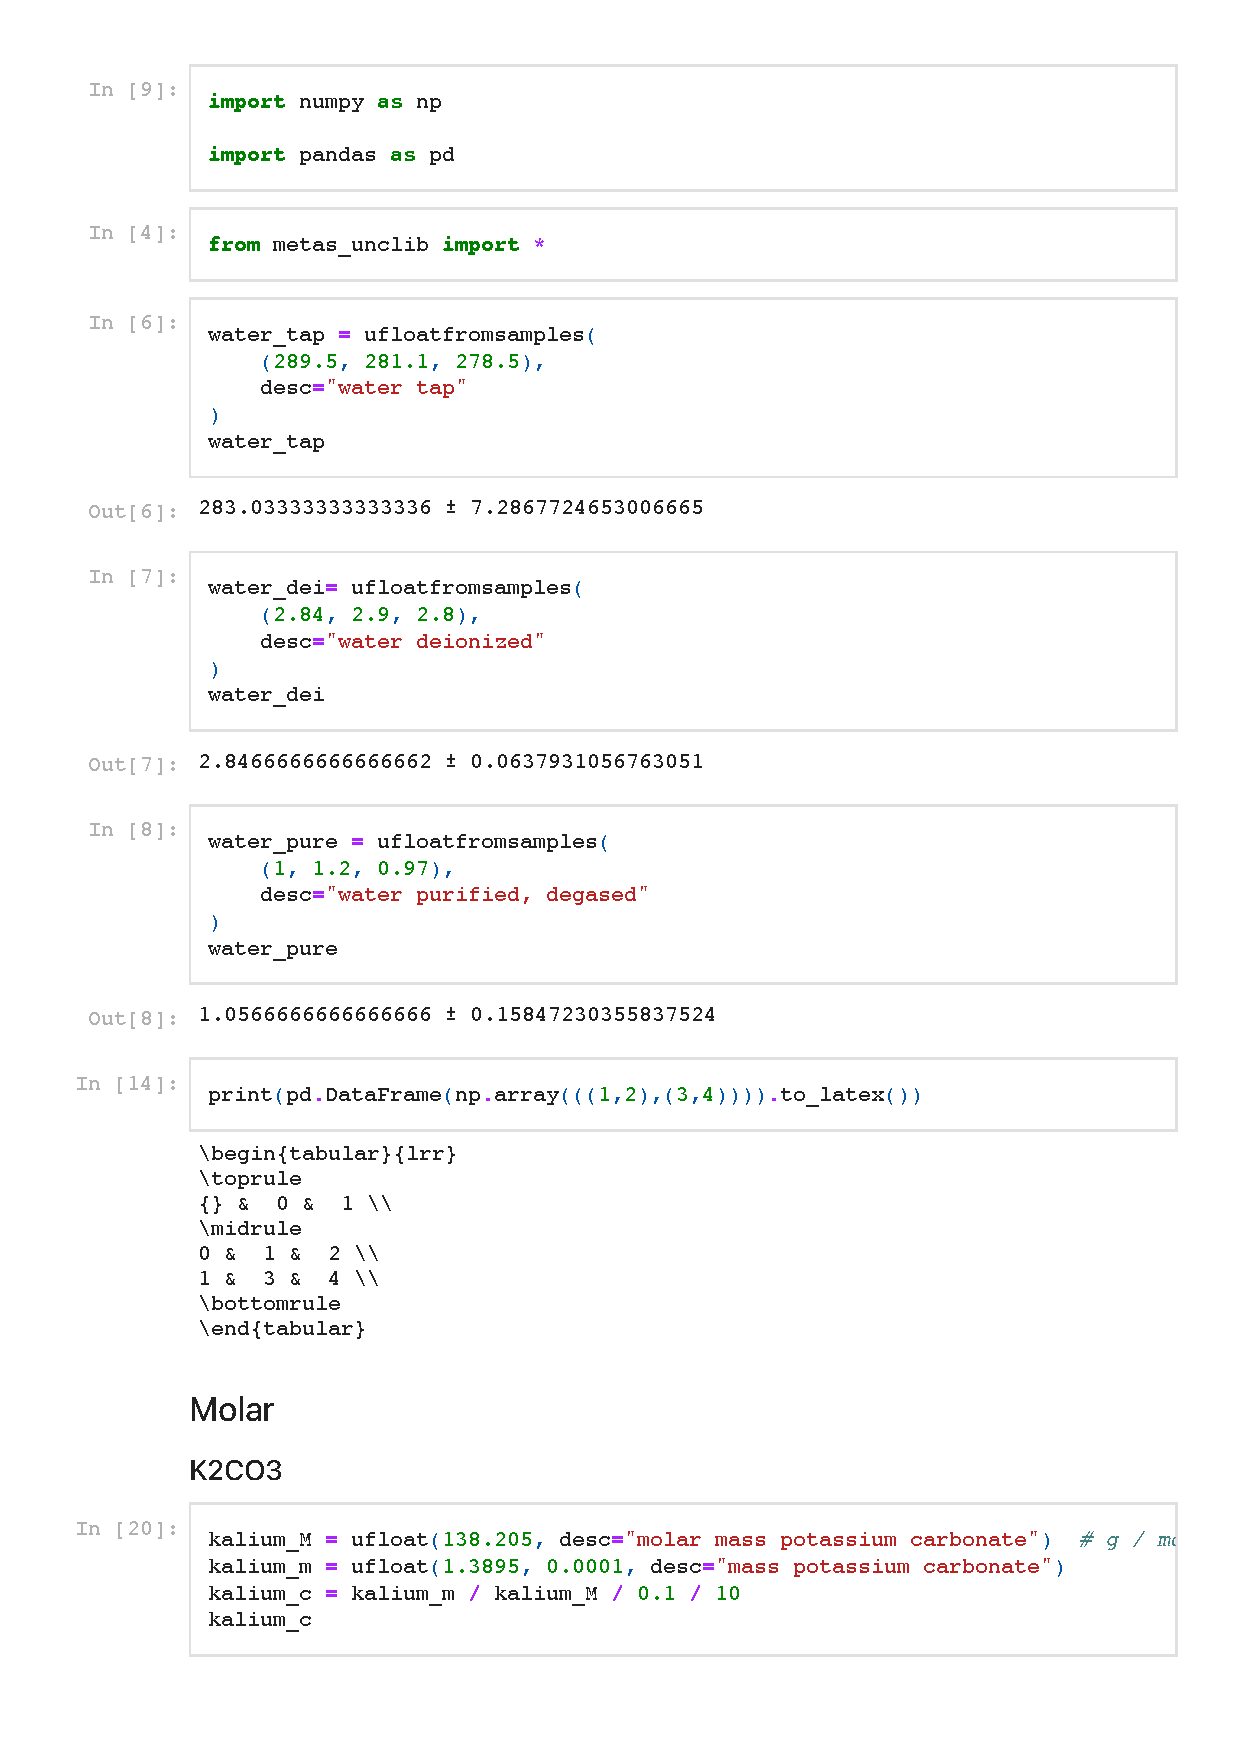
\includepdf[pages=1, scale = 0.75, pagecommand=\subsubsection{Conductivity of differently treated water samples and molar conductivity of different electrolytes}]{scripts/LFK_water_and_molar.pdf} 
\includepdf[pages=2-, scale = 0.75,pagecommand={}]{scripts/LFK_water_and_molar.pdf} \label{append:LFK_water_and_molar}


\iffalse{

\subsubsection{Vapor Pressure Analysis}
\Rfile{scripts/DDR1_shared_plot.R}
%\inputminted{R}{scripts/DDR1_shared_plot.R}
% \caption{Auswertungsskript Dampfdruckkurve}

\newpage
\subsubsection{\texttt{TREVAC} Analysis}
\Rfile{scripts/DDR2.R}


\newpage

\begin{figure}[H]
    \centering
    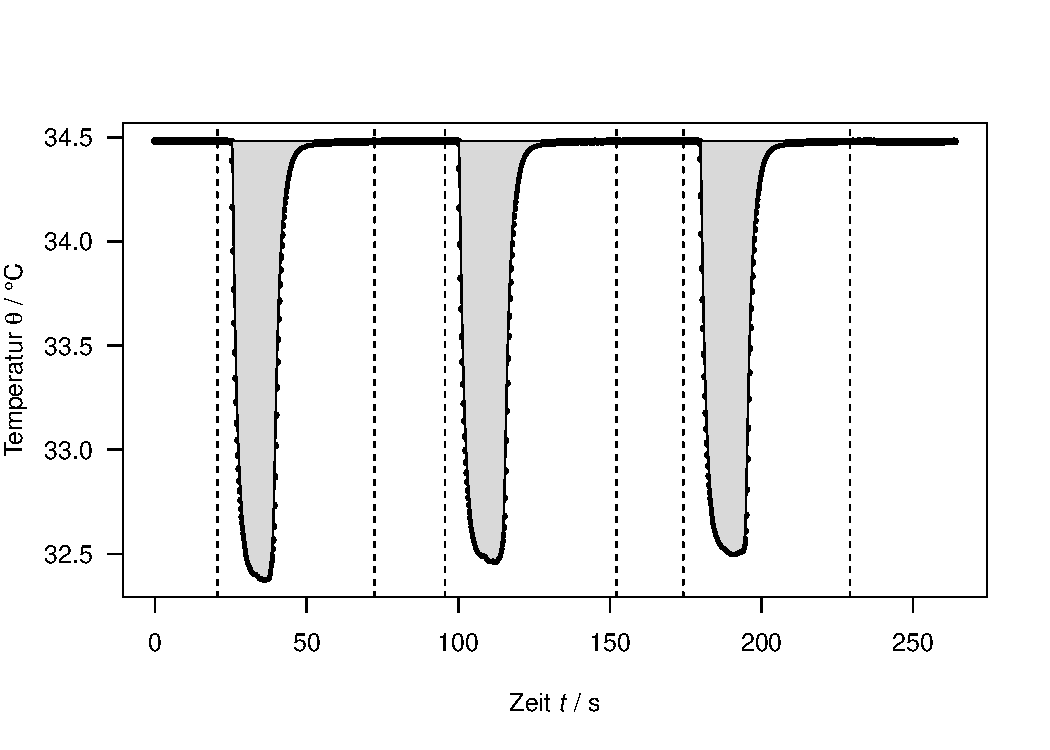
\includegraphics[width=.5\textwidth]{figures/methanol.pdf}
    \caption{\texttt{TREVAC} area analysis of methanol as reference value.}
    \label{fig:sketch_rho}
\end{figure}

\begin{figure}[H]
    \centering
    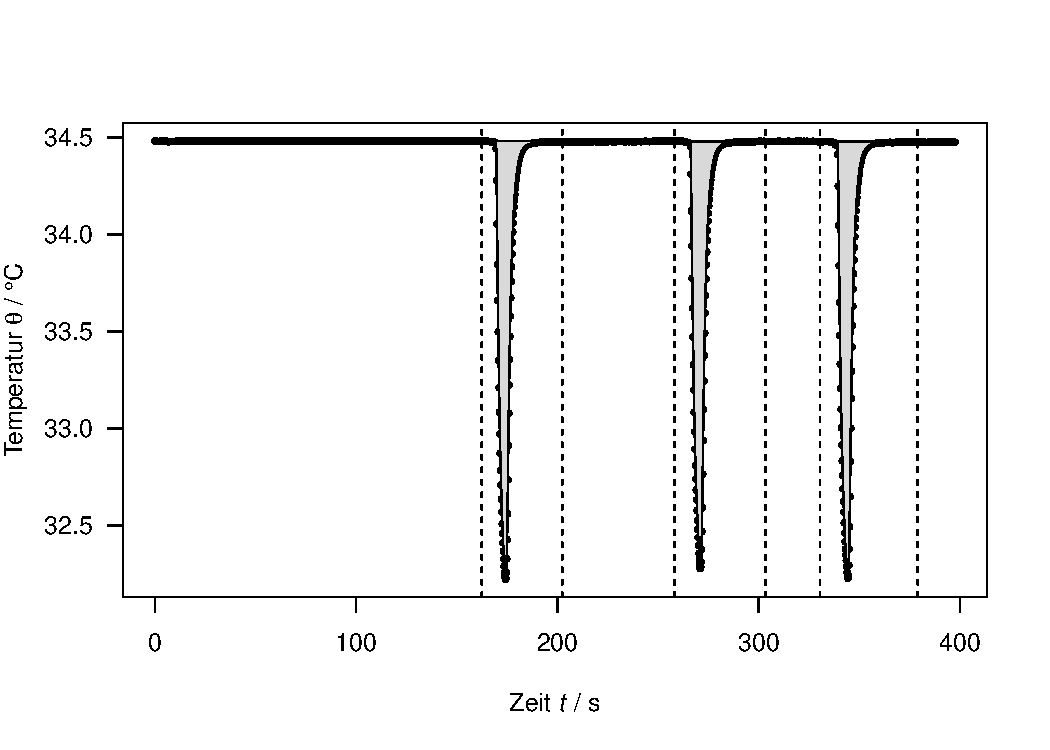
\includegraphics[width=.5\textwidth]{figures/acetone.pdf}
    \caption{\texttt{TREVAC} area analysis of acetone.}
    \label{fig:sketch_rho}
\end{figure}

\begin{figure}[H]
    \centering
    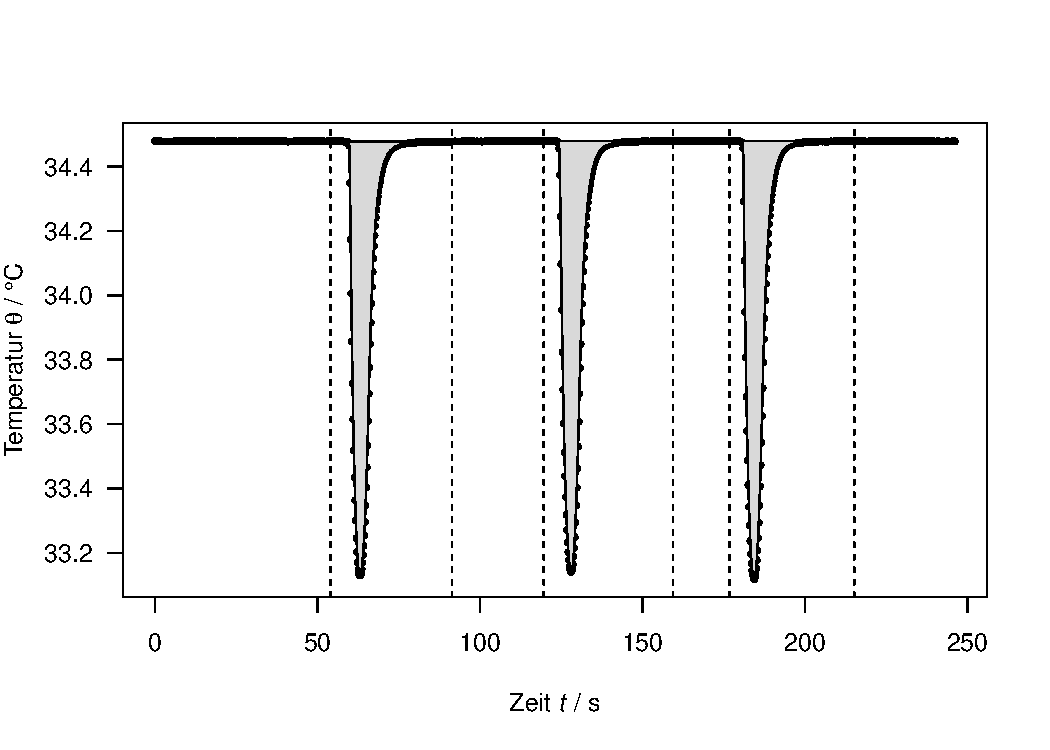
\includegraphics[width=.5\textwidth]{figures/n-hexane.pdf}
    \caption{\texttt{TREVAC} area analysis of n-hexane.}
    \label{fig:sketch_rho}
\end{figure}


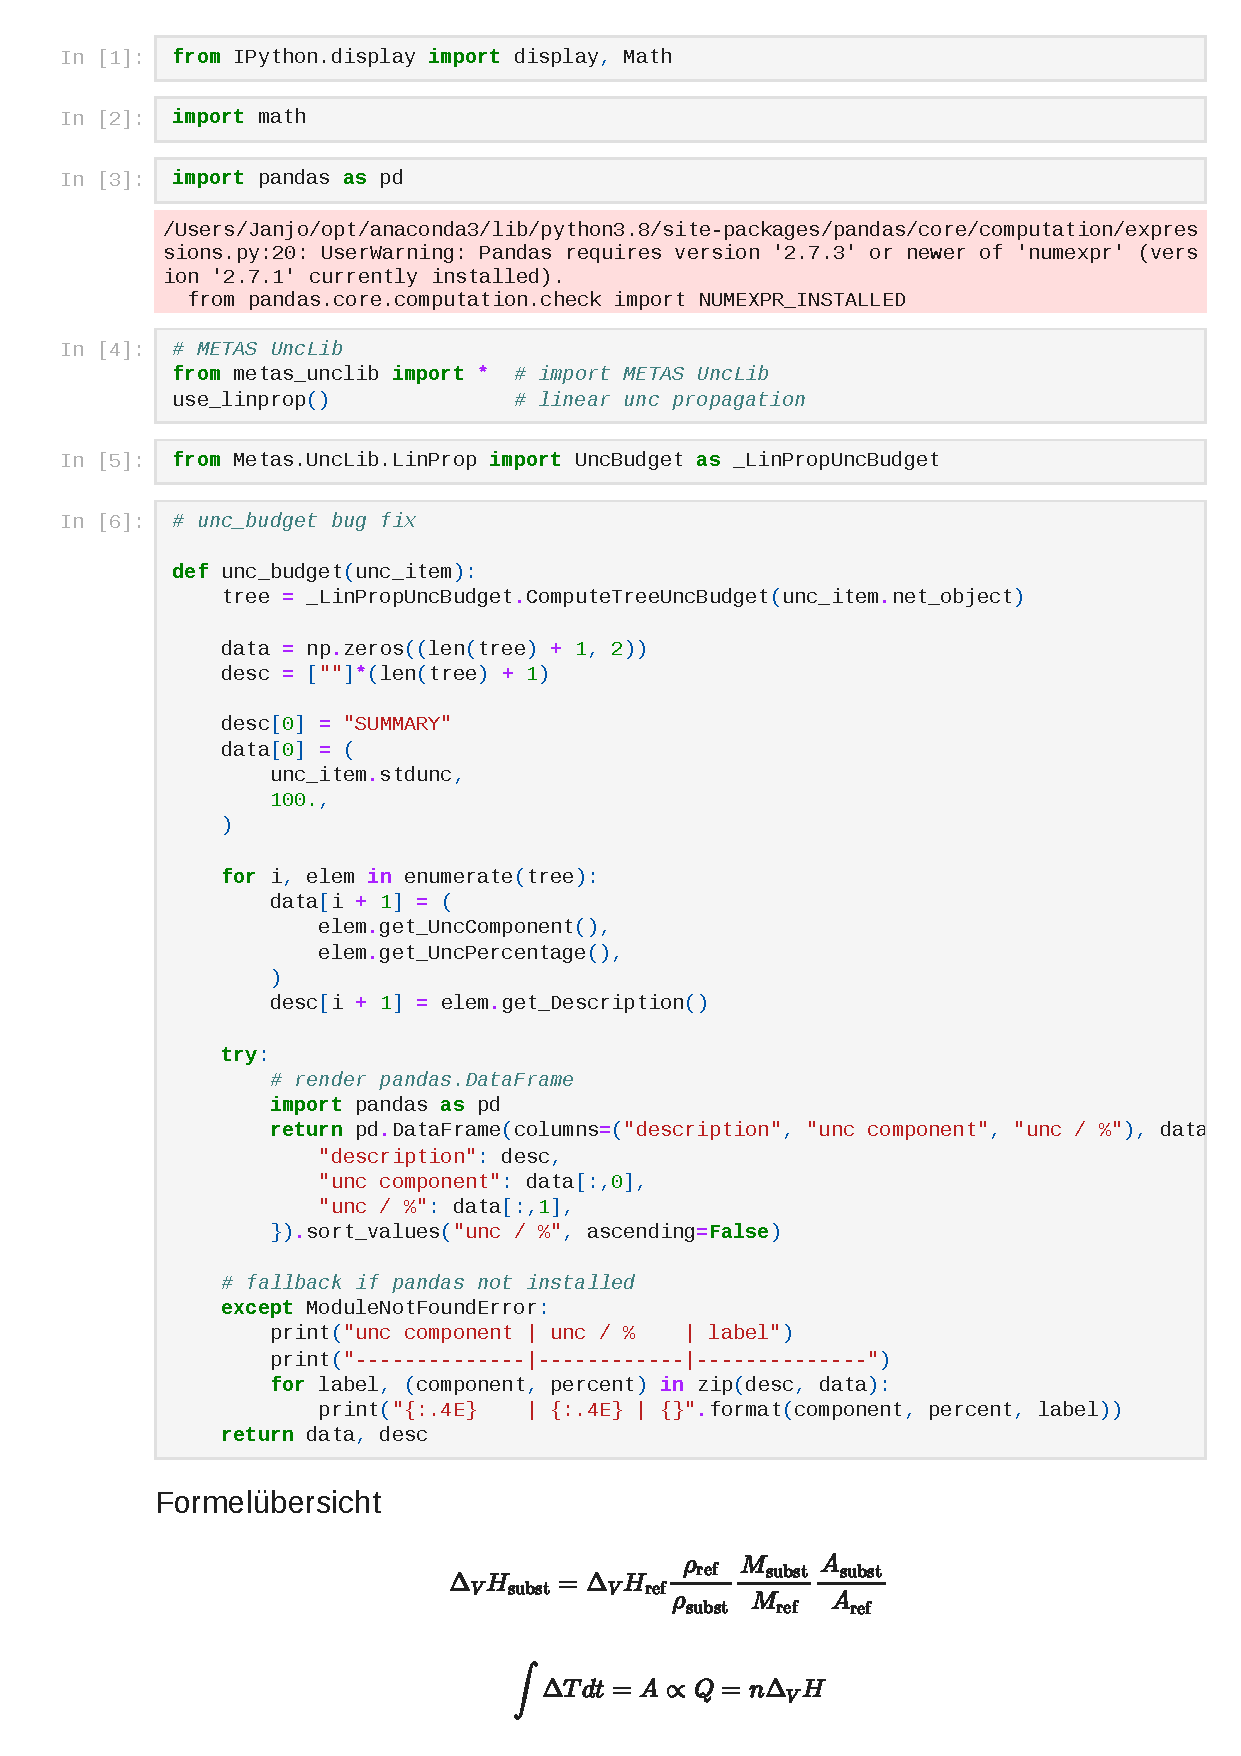
\includepdf[pages=1, scale = 0.75, pagecommand=\subsubsection{TREVAC results and uncertainty estimates}]{scripts/metas_unclib_ddr2.pdf} 
\includepdf[pages=2-, scale = 0.75,pagecommand={}]{scripts/metas_unclib_ddr2.pdf} \label{lab_journal}

\newpage
\subsubsection{Density comparison plot}
\Rfile{scripts/rho_comparisons.R}

\newpage
\subsubsection{Plotting helper scripts}
\Rfile{scripts/helpers.R}

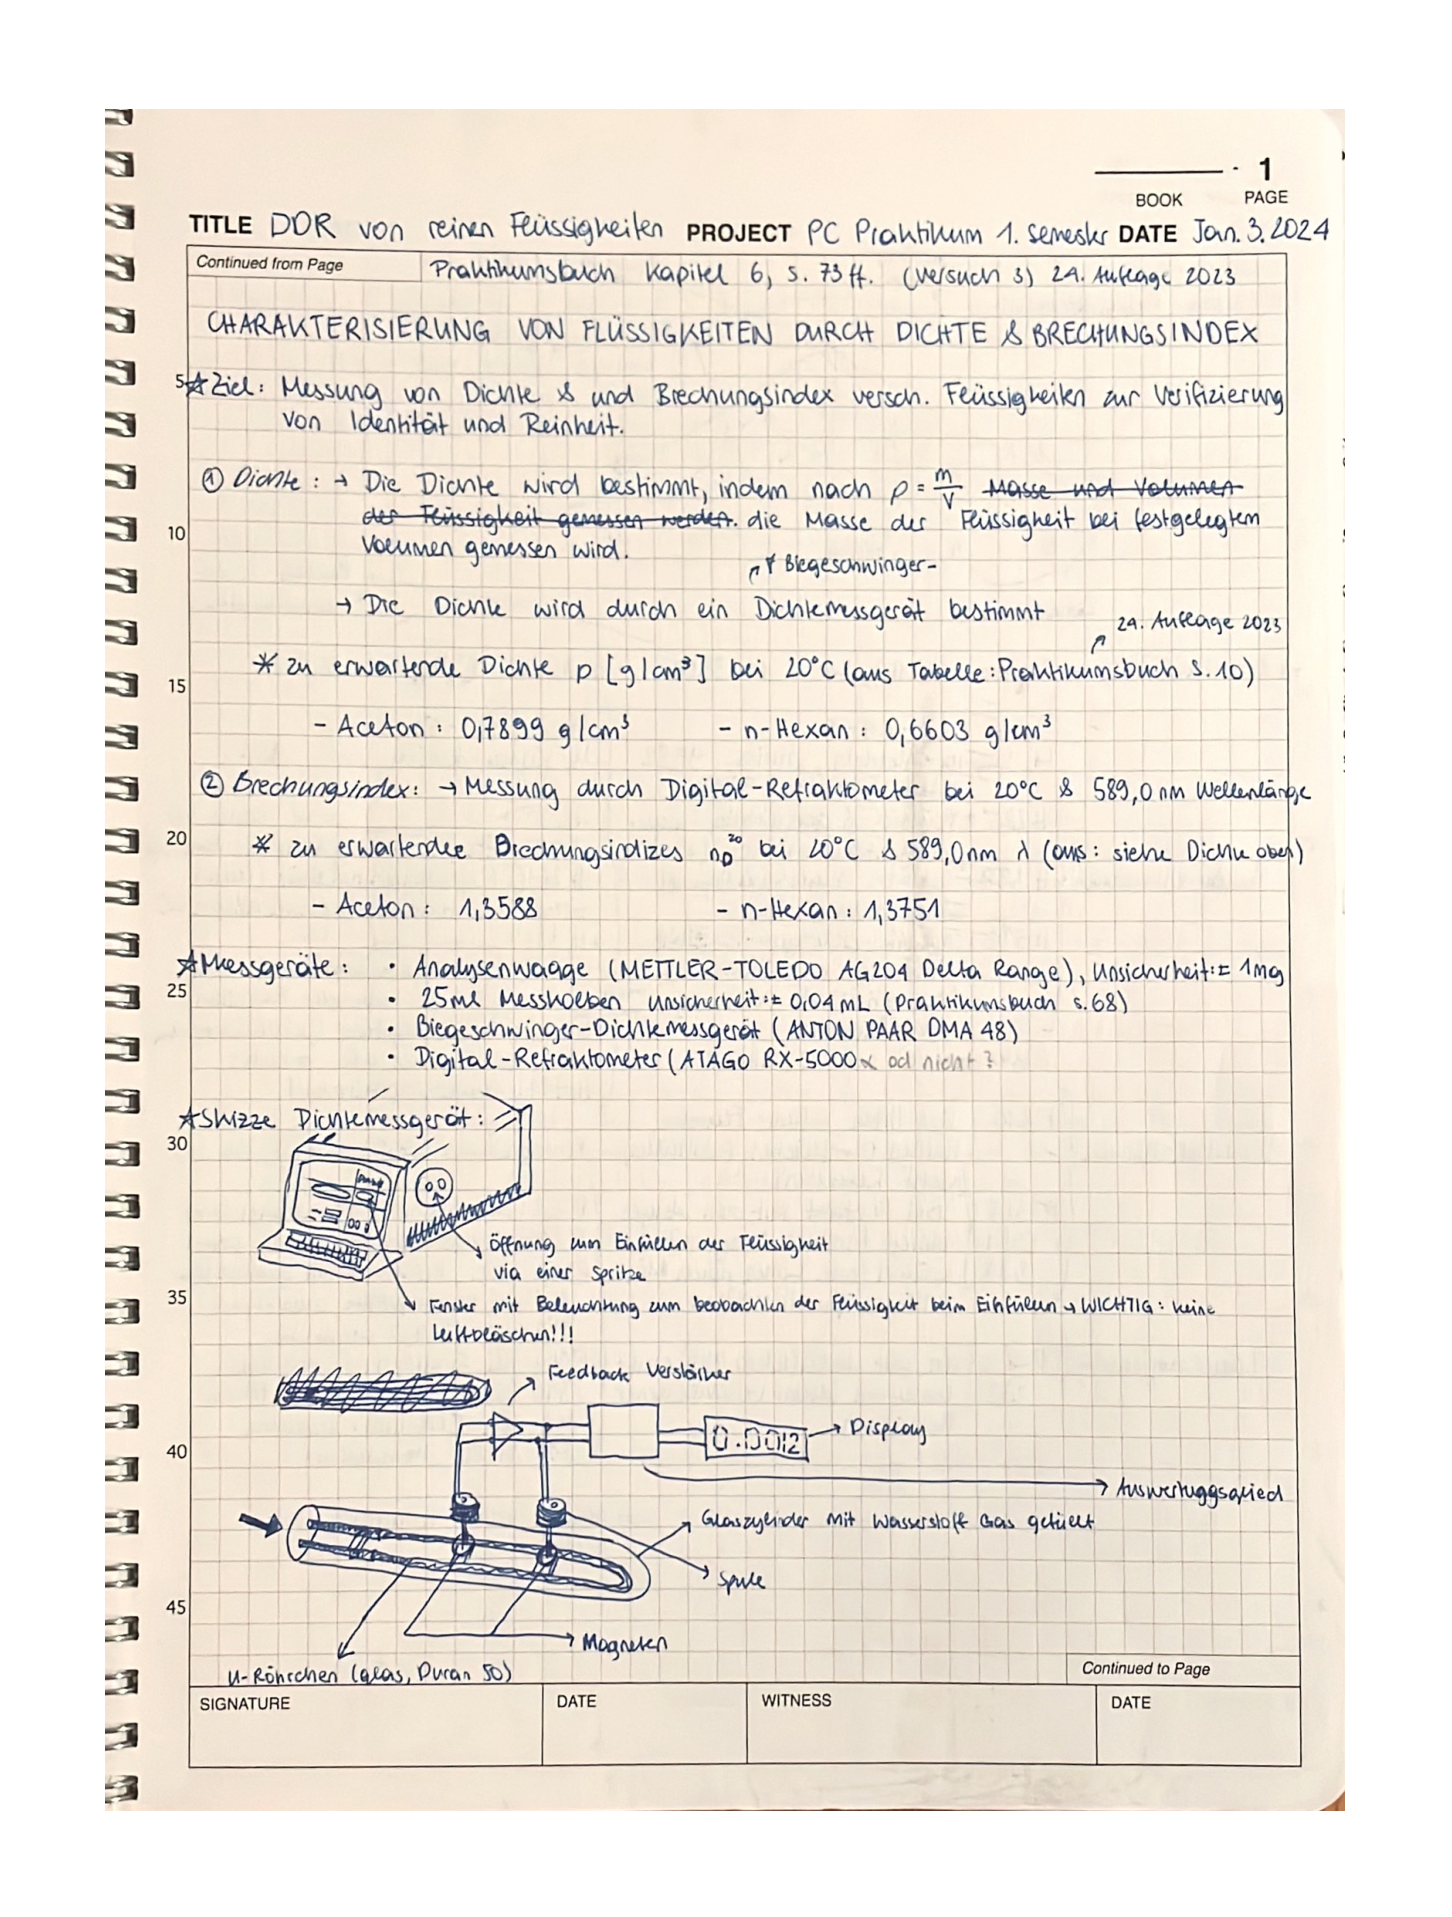
\includepdf[pages=1, scale = 0.75, pagecommand=\subsection{Lab Journals}]{figures/ddr_lab_journal.pdf} 
\includepdf[pages=2-, scale = 0.75,pagecommand={}]{figures/ddr_lab_journal.pdf} \label{lab_journal}



\lstinputlisting[caption=Automatic rounding functions to fit the 25 rule of the significant digits.]{scripts/25Utils.R}
\lstinputlisting[inputencoding=utf8/latin1, caption=Code for the evaluation of the first experiment: Enthalpy of evaporation.]{scripts/DDR.R}
\lstinputlisting[inputencoding=utf8/latin1, caption=Code for the evaluation of the second experiment: Transient evaporation cooling.]{scripts/DDR2.R} \label{ddr_code2}

\includepdf[pages=1, scale = 0.75, pagecommand=\subsection{Lab journal copies}]{figures/LabJournalDDR.pdf} 
\includepdf[pages=2-, scale = 0.75,pagecommand={}]{LabJournalDDR.pdf} \label{lab_journal}

\includepdf[pages=1, scale = 0.75, pagecommand=\subsection{Exercises from the script}]{figures/U_DDR.pdf}
\includepdf[pages=2-, scale = 0.75,pagecommand={}]{U_DDR.pdf}

\subsection{Additional data plots}

\subsubsection{Transistent evaporation cooling}

\begin{figure}[H]
    \centering
    \subfigure[]{\includegraphics[width=.49\textwidth]{figures/DDR2_cyc.pdf}}
    \subfigure[]{\includegraphics[width=.49\textwidth]{DDR2_pol.pdf}}
    \caption{Profile of the evaporation of 5 $\mu$L of (a) Cyclohexane and (b) 1-Propanol.}
    \label{fig:ddr2_appendix}
\end{figure}

\subsection{Safety}

The Hazards-\&Precautionary phrases were copied from data sheets found at \cite{Sigma-Aldrich}.

\subsubsection{Cyclohexane}
\ghspic[scale = 0.75]{flame} \ghspic[scale = 0.75]{acid} \ghspic[scale = 0.75]{exclam} \ghspic[scale = 0.75]{aqpol} \\

\noindent
\ghs{h}{225} \\
\ghs{h}{304} \\
\ghs{h}{315} \\
\ghs{h}{336} \\
\ghs{h}{410} \\
\ghs{p}{210} \\
\ghs{p}{233} \\
\ghs{p}{273} \\
\ghs{p}{301+310}\\
\ghs{p}{303+361+353}\\
\ghs{p}{331} \\

\subsubsection{1-Propanol}
\ghspic[scale = 0.75]{flame} \ghspic[scale = 0.75]{acid} \ghspic[scale = 0.75]{exclam} \\

\noindent
\ghs{h}{225} \\
\ghs{h}{318} \\
\ghs{h}{336} \\
\ghs{p}{210} \\
\ghs{p}{233} \\
\ghs{p}{240} \\
\ghs{p}{241} \\
\ghs{p}{280} \\
\ghs{p}{305+351+338}\\

\subsubsection{Methanol}
\ghspic[scale = 0.75]{flame} \ghspic[scale = 0.75]{skull} \ghspic[scale = 0.75]{health}

\noindent
\ghs{h}{225} \\
\ghs{h}{301}+\ghs{h}{311}+\ghs{h}{331} \\
\ghs{h}{370} \\
\ghs{p}{210} \\
\ghs{p}{233} \\
\ghs{p}{280} \\
\ghs{p}{301}+\ghs{p}{310} \\
\ghs{p}{303}+\ghs{p}{361}+\ghs{p}{353} \\
\ghs{p}{304}+\ghs{p}{340}+\ghs{p}{311} \\


}